\documentclass[a4paper]{article}

\usepackage[english]{babel}
\usepackage[utf8x]{inputenc}
\usepackage{amsmath}
\usepackage{amsfonts}
\usepackage{graphicx}
\usepackage[colorinlistoftodos]{todonotes}

\title{CS 5785 -- Applied Machine Learning -- Lec.\ 8}
\author{Prof.\ Nathan Kallus, Cornell Tech\\Scribe: TBD}
\date{Sept.\ 19, 2017}

\begin{document}
\maketitle

\section{Singular Value Decomposition}

\subsection{Review from Last Time}
Recall that the SVD decomposes a rectangular matrix ${\mathbf X}\in {\mathbb R}^{N\times p}$ into the product of three matrices $\mathbf{X}=\mathbf{UD}\mathbf{V}^\top$ where:
\begin{itemize}
\item ${\mathbf U}\in {\mathbb R}^{N\times p}$: Matrix of the left singular vectors.
\item ${\mathbf V}\in {\mathbb R}^{p\times p}$: Matrix of the right singular vectors.
\item ${\mathbf D}=diag\{d_1,d_2,\ldots, d_p\}\in {\mathbb R}^{p\times p}$, where for all the singular values it holds that $d_1\geq d_2\geq \ldots \geq d_p \geq 0$.
\end{itemize}
$\mathbf{U}$ and $\mathbf{V}$ both have orthogonal columns, so $\mathbf{U}^\top\mathbf{U}=\mathbf{I}$ and $\mathbf{V}^\top\mathbf{V}=\mathbf{I}$ where $\mathbf{I}$ is the identity matrix of size $p\times p$.

We can also write the SVD as a sum of outer products: $$\mathbf{X}=\mathbf{UD}\mathbf{V}^\top=\sum_{j=1}^pd_ju_jv_j^\top$$
Where $u_j$ and $v_j$ are the  $j^{th}$ columns of $\mathbf{U}$ and $\mathbf{V}$, respectively. Thus the SVD expresses a matrix as a sum of rank $1$ matrices weighted by the scalars $d_j$.

The clown image in Figure 1 example from the last lecture shows examples of this sum truncated at 2, 5 and 20 terms, yielding approximations of the image of increasing quality, similar to different levels of image compression.  Figure \ref{fig:sval_plot} illustrates how the singular values fall off for this image; this indicates that there is a lot of redundancy in the rows/columns.  (Note the log scale on the vertical axis.)  An image formed by randomly shuffling the pixels of the clown image, on the other hand, exhibits relatively little redundancy between its columns/rows and this is reflected in the singular values falling off slowly. As such, a completely random generated matrix is usually full rank. This is an important characteristic of the SVD: a natural image would produce high redundancy whereas a randomly generated image would be far less redundant. 

\begin{figure}
\centering
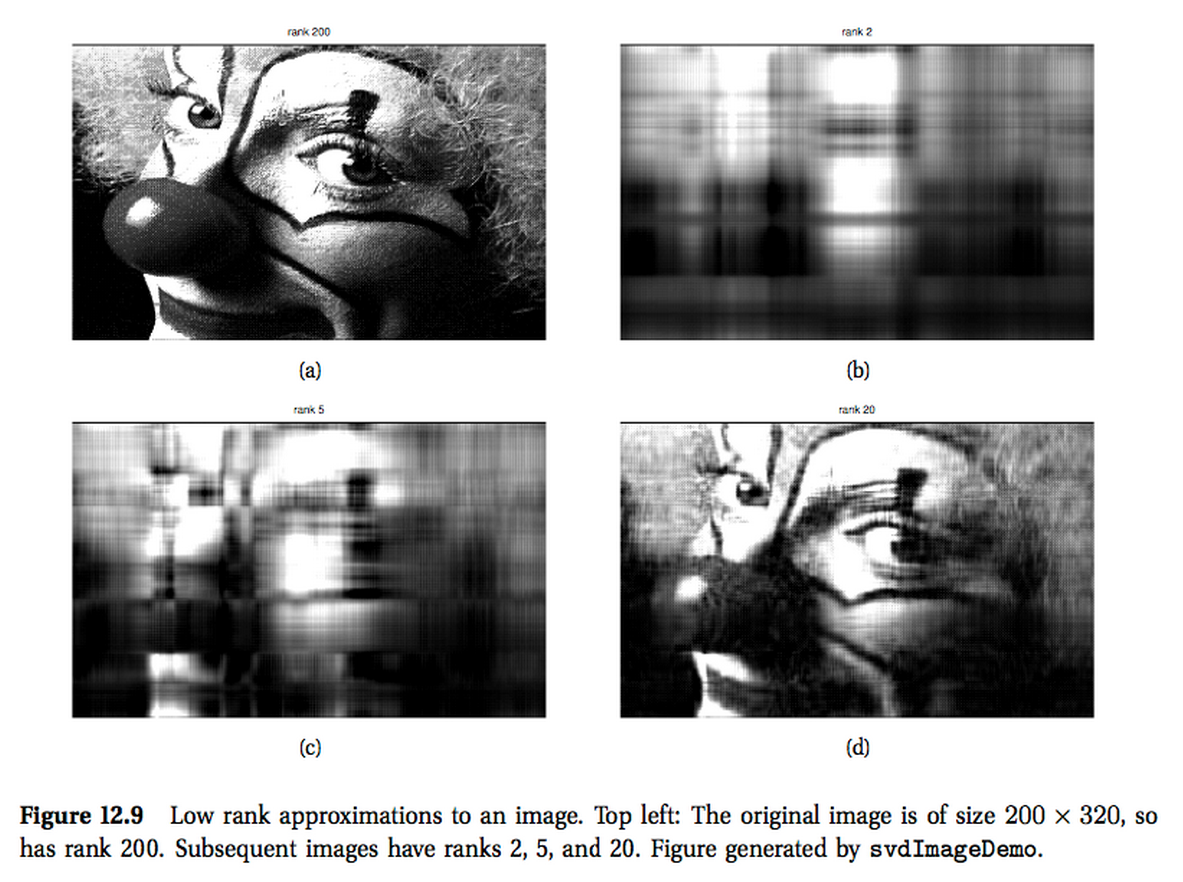
\includegraphics[width=1.0\textwidth]{clown_example.png}
\caption{\label{fig:clown_example}[Murphy]}
\end{figure}

\begin{figure}
\centering
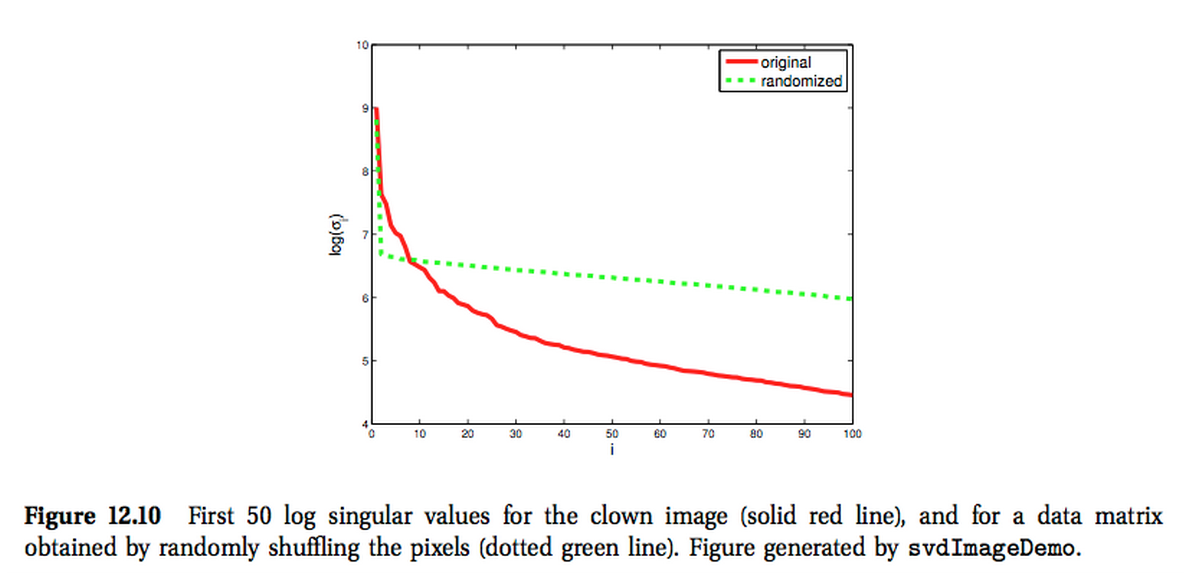
\includegraphics[width=1.0\textwidth]{sval_plot.png}
\caption{\label{fig:sval_plot}[Murphy]}
\end{figure}


\subsection{Consequences of Orthogonality}
Using the identity $(\mathbf{A}\mathbf{B}\mathbf{C})^\top=\mathbf{C}^\top\mathbf{B}^\top\mathbf{A}^\top$,
\begin{eqnarray*}
\mathbf{X}^\top \mathbf{X} &=& \mathbf{VD}\mathbf{U}^\top\mathbf{UD}\mathbf{V}^\top\\
 &=& \mathbf{VDD}\mathbf{V}^\top\\
 &=& \mathbf{V}\mathbf{D}^{2} \mathbf{V}^\top
\end{eqnarray*}
This is the eigendecomposition of $\mathbf{X}^\top \mathbf{X}$, which is $p\times p$.  Similarly, one can show,
\begin{eqnarray*}
\mathbf{X}\mathbf{X}^\top &=& \mathbf{U}\mathbf{D}^{2} \mathbf{U}^\top
\end{eqnarray*}
This is the eigendecomposition of $\mathbf{X} \mathbf{X}^\top$, which is $N\times N$.  From this we see that $\mathbf{X}\mathbf{X}^\top$ and $\mathbf{X}^\top\mathbf{X}$ have the same eigenvalues. 
%In many cases, $p\ll N$, i.e., the dimensionality of the data is much smaller than the number of examples, and this means one of these matrices is huge and the other is small.

The two square, symmetric matrices $\mathbf{X}^\top \mathbf{X}$ and $\mathbf{X} \mathbf{X}^\top$ are \emph{positive semidefinite} by construction, which means all the eigenvalues are non-negative.  Think of positive semidefiniteness as a matrix counterpart to positivity for scalars.  If a scalar $a$ is known to be the product of another (real valued) scalar $q$ with itself, i.e., $a=q\cdot q=q^2$, then we know $a$ will be nonnegative, by construction, regardless of the value of $q$.  Analogously, if we define a matrix $\mathbf{A}$ as a product of a matrix $\mathbf{Q}$ with its transpose, i.e., $\mathbf{A}=\mathbf{Q}\mathbf{Q}^\top$ or $\mathbf{A}=\mathbf{Q}^\top\mathbf{Q}$, the eigenvalues\footnote{Note: positive semidefinite does not mean all the \emph{entries} in $\mathbf{A}$ are nonnegative, but rather that all the \emph{eigenvalues} of $\mathbf{A}$ are nonnegative.} of $\mathbf{A}$ will be nonnegative, by construction, regardless of the values in $\mathbf{Q}$.  (We leave the proof of this as an exercise.)  Covariance matrices are important examples of positive semidefinite matrices. That makes sense since it would be weird for the variance to be negative or complex.

\subsection{Computing Eigenvectors of Large Matrices}
Given a matrix ${\mathbf B}$ and a vector $a$, the \emph{Rayleigh quotient} is defined as:
$$
\frac{a^\top {\mathbf B} a}{a^\top a}
$$
In the numerator we have the quadratic form $a^\top {\mathbf B} a$ and in the denominator we have $a^\top a$, which is simply $\|a\|^2$, the squared norm of $a$.  Dividing out the norm has the effect of normalizing the expression, so without loss of generality, we can think of $a$ as having unit norm.  Now consider the set of all possible vectors $a$: the choice of $a$ that maximizes the Rayleigh quotient is the leading eigenvector of $\mathbf{B}$.  The value attained at the maximum is the corresponding eigenvalue.  This leading eigenvector represents the dimension along which the data exhibits the most spread. For successive eigenvectors, we repeat the maximization procedure on $a$ with the constraint that they be orthogonal to the previous eigenvectors. 

What happens if you want to do the SVD on really large matrices?  In many cases of practical interest, we only need a relatively small set of leading eigenvectors/singular vectors.  We observed this, for example, in the clown image in Figure \ref{fig:clown_example}, for which the singular values drop off dramatically (Figure \ref{fig:sval_plot}, red line).  Going from one row to the next in this image, the pixel values don't change very much.

\subsubsection{Power Iteration}

Suppose we have $\mathbf{B} = \mathbf{X}^\top \mathbf{X}$ and we want the leading eigenvector. Let $\mathbf{\Lambda} = \mathbf{D}^2$ and $\mathbf{B} = \mathbf{V} \mathbf{\Lambda} \mathbf{V}^\top$. Pick a random vector $a_k$ and iterate on
$$
a_{k+1} = \frac{\mathbf{B} {a_k}}{\|\mathbf{B} {a_k}\|}
$$
In general, multiplying a matrix $\mathbf{A}$ by a vector $a$ does two things to that vector: it rotates and scales it.  If you choose $a$ to be an eigenvector of $\mathbf{A}$, something special happens: $\mathbf{A}$ just scales the vector by a constant. If you repeat the iteration defined above, you will eventually converge to an eigenvector.  Why does this work?  Effectively, we are multiplying $a_k$ by higher and higher powers of $\mathbf{B}$.  Observe what happens when we raise $\mathbf{B}$ to a high power:
\begin{eqnarray*}
\mathbf{B}^n &=& (\mathbf{V} \mathbf{\Lambda} \mathbf{V}^\top)^n \\
&=& (\mathbf{V} \mathbf{\Lambda} \mathbf{V}^\top)(\mathbf{V} \mathbf{\Lambda} \mathbf{V}^\top)\cdots(\mathbf{V} \mathbf{\Lambda} \mathbf{V}^\top) \\
&=& \mathbf{V} \mathbf{\Lambda}^n \mathbf{V}^\top
\end{eqnarray*}
In other words, the exponent $n$ moves inside the diagonalization to sit on $\mathbf{\Lambda}$, the diagonal matrix of eigenvalues ($\lambda_1, \lambda_2, \ldots$ in descending order).  Now suppose we divide all the eigenvalues by $\lambda_1$.  This will make the first entry $1$ and all the rest less than $1$.  If you raise all these numbers to the $n^{th}$ power, the other values will eventually get driven to $0$ if there's a gap between $\lambda_1$ and the rest of the eigenvalues.  After many iterations, we get a rank $1$ matrix $v_1 v_1^\top$, from which we can easily extract the leading eigenvector.

What causes trouble for power iteration?
If the gap between the first eigenvalue and the next ones is really small, it will take a very long time to drive the next eigenvalue to 0.  The pathological case would be a gap of zero, i.e., repeated eigenvalues.  This is called a subspace and power iteration will break.  To avoid problems such as repeated eigenvalues and also to exploit properties of large matrices that are sparse, we use tools such as inverse iteration or the Lanczos Method, which is well-suited to Map-Reduce implementation.  Inverse iteration was developed as a followup to power iteration that can handle subspaces of size $k$.  A sparse matrix is a matrix with lots of zeros which could represent, for example, the vast quantities of movies or songs users have not rated on sites such as Netflix or Pandora that make extensive use of recommender systems.  (It's not realistic to assume users on such sites can rate every item).

\section{Kernel Smoothing}
Kernel smoothing is an idea from statistics in which we use weighted averages to smooth noisy, irregularly spaced training data.  When you have a finite sample of data as depicted in Figure \ref{fig:fig6_1}, you may have reason to believe there's an underlying smooth signal for which your finite sample represents. Kernel smoothing helps you obtain a continuum,  if you want to look up a function value at a point where you didn't sample any data, kernel smoothing can give you an answer.

\begin{figure}
\centering
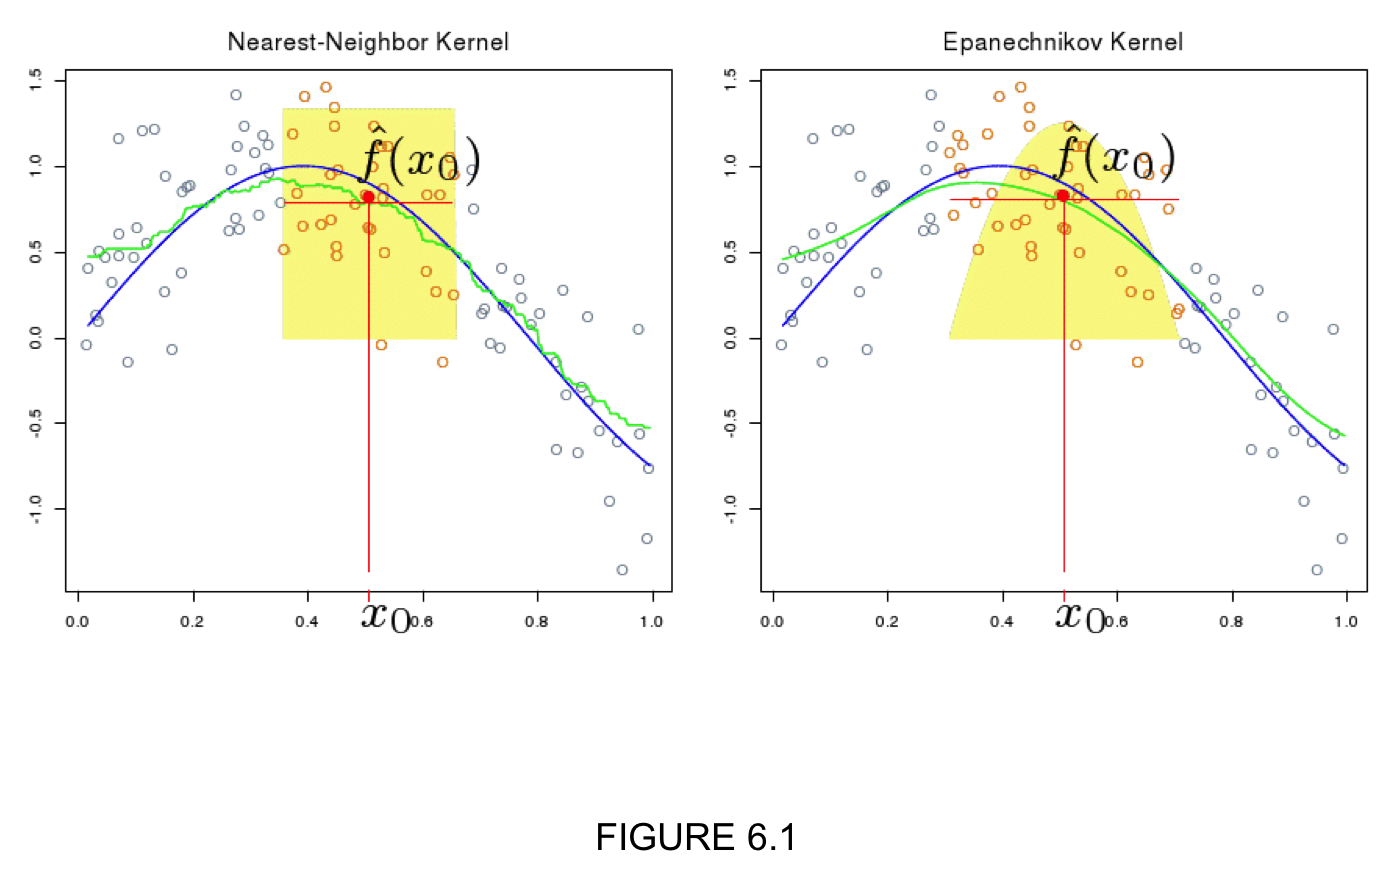
\includegraphics[width=1.0\textwidth]{fig6_1.png}
\caption{\label{fig:fig6_1}[Kernel Smoothing]}
\end{figure}

%Smoothing signals would involve some value being tracked over time.  There's nothing probabilistic about it: just noisy data over time getting smoothed.

%Smoothing density data is smoothing samples so if you have an exam that 100 students get scores for.  You have instances of this random variable.  For instance you might create a histogram.

Suppose you want to smooth noisy sensor measurements that are a function of time.  One method is $k$ nearest neighbor smoothing:
$$\widehat{f}(x) = Ave\left(y_i | x_i \in N_k(x)\right)$$
This is an estimate of the regression function $E(Y|X=x)$ where $N_k(x)$ is the set of $k$ points closest to $x$ and $Ave$ computes the mean.  This is what's happening in the Figure \ref{fig:fig6_1}(left).  In other words, the $k$-NN smoother estimates $\widehat{f}(x_0)$ at some arbitrary value $x_0$ using the average value of the $k$ nearest neighbors of $x_0$. In Figure \ref{fig:fig6_1}, the blue curve represents the ground truth curve from which the noisy samples were obtained.  The result of the $k$-NN smoother is shown by the green line in the plot on the left.  This method, though simple, generally yields a jumpy discontinuous curve, which is undesirable.  As the window moves, one point is added and one point is left out, which leads to the jumpy behavior. The window is depicted by the yellow region in the left image in Figure 3.

Kernel smoothers address this problem by using a weighting function that dies off smoothly toward the edges. Thus, the smoothing function pays more attention to data points closer to the target point and less attention to data points further away. We express this as follows:
$$\widehat{f}(x_0) = \frac{\sum_{i=1}^{N} K_\lambda (x_0, x_i) y_i}{\sum_{i=1}^{N} K_\lambda (x_0, x_i)}$$

$$K_\lambda (x_0, x) = D\left(\frac{|x-x_0|}{\lambda}\right)$$

$$D(t) = \begin{cases}
    \frac{3}{4}({1-t^2}),& \text{if } |t|\leq 1\\
    0,              & \text{otherwise}
\end{cases}$$
In this case, we have chosen $D(\cdot)$ to be an \emph{Epanechnikov kernel}, which has a quadratic shape within a fixed interval.  In this case, you pick a particular width, $\lambda$, and you perform a weighted average of the $y$ values in the corresponding interval, paying more attention to the data near the center.  Weighting the y values lets points closest to the center have the greatest influence, instead of all points having the same impact, as in the $k$-NN smoother. This results in a smoother curve, shown in green on the right of Figure \ref{fig:fig6_1}.  The yellow part in the right image in Figure 3 depicts the chosen window of this fancy weighted average.

Note, this isn't necessarily any more accurate than what we obtained from the $k$-NN smoother, though it may be qualitatively better.  What matters is its utility in real world applications, i.e., its ability to predict subsequent data.

This idea of kernel smoothing can also be applied to density estimation, which is discussed in the next lecture.

\end{document}
